\documentclass{acm_proc_article-sp}

\begin{document}

\title{A Method Based on Interactive Evolutionary Computation for
  Increasing the Effectiveness of Advertisement Texts for Clusters of People}

\numberofauthors{3}

\author{
\alignauthor
Quetzali Madera\\
       \affaddr{Tijuana Institute of Technology}\\
       \affaddr{Calzada Tecnologico s/n, Tomas Aquino}\\
       \affaddr{Tijuana, Mexico}\\
       \email{quetzalimadera@ tectijuana.edu.mx}
\alignauthor
Mario Garc\'ia-Valdez\\
       \affaddr{Tijuana Institute of Technology}\\
       \affaddr{Calzada Tecnologico s/n, Tomas Aquino}\\
       \affaddr{Tijuana, Mexico}\\
       \email{mario@tectijuana.edu.mx}
\alignauthor
Alejandra Mancilla\\
       \affaddr{Tijuana Institute of Technology}\\
       \affaddr{Calzada Tecnologico s/n, Tomas Aquino}\\
       \affaddr{Tijuana, Mexico}\\
       \email{alejandra.mancilla@gmail.com}
}

\maketitle
\begin{abstract}
Interactive Evolutionary Computation (IEC) is used in this work in
order to perform the optimization of several advertisement blocks of
text. The advertisement texts follow a format
similar to the one used in a technique called Article Spinning. This
format allows an IEC algorithm to evolve the text for a certain
cluster of people, using words and phrases as variable
parts which change according to the subjective evaluation of the
corresponding cluster of people interacting with the algorithm. After
several generations, the IEC algorithm provides a version of the
advertisement text that, in theory, should exhibit an increased
performance, according to the subjective evaluation function it was
evolved with. In order to demonstrate the efficiency of the texts,
these are compared against a version determined by an expert in a
field related to marketing. For this comparison, three tests are
performed: recall, recognition, and persuasion tests. The results
obtained show that IEC could effectively be used to increase the
impact of an advertisement text, but more experiments need to be
conducted. A recommendation of an advertisement text is accomplished
by determining an individual's corresponding cluster, and showing an
evolved version of the text for that particular cluster.
\end{abstract}

\category{H.4}{Information Systems Applications}{Miscellaneous}
\category{D.2.8}{Software Engineering}{Metrics}[complexity measures, performance measures]
\terms{Theory}

\keywords{ACM proceedings, \LaTeX, text tagging}

\section{Introduction}

This paper presents a method for optimising advertisement
texts through the use of Interactive Evolutionary Computation (IEC)
techniques, and a method for the recommendation of these texts based
on clustering algorithms. The advertisiment texts can be of arbitrary length, but
short texts are used in the conducted experiments. For an
advertisement text to be evolved, it needs to follow a proposed
format, described in Section \ref{ArticleSpinning}. This format allows
the representation of the text as a chromosome that can be used by a
genetic algorithm (see Section \ref{GeneticAlgorithms}) for its evolution.

The texts are evolved in different environments or habitats, defined
by a clustering algorithm. Before individuals interact with the
IEC algorithm, a clustering algorithm will decide to what cluster these
users belong to, based on their profile. After determining a user's cluster, the user can then
interact with the evolution process (see Section
\ref{EvolutionProcess}). The number of habitats where the texts will
be evolving will depend on the predefined number of clusters.

\subsection{Justification}

The reason for the development of the proposed method in this work is
the potential to lower monetary costs in advertisement campaigns and
simplification of advertisement logistics.

For example, this method could be implemented in a website. The
profiles of the users could be obtained using their Facebook profiles' information,
and user clusters would be created based on this information. Visitors
would be assigned to a cluster and would participate in the
evolutionary process of the advertisement texts whenever they decide
to click on certain advertisements, or ignore them. The website's
visitors would be optimizing their own advertisements.

\section{Basic Concepts}

\subsection{Genetic Algorithms}
\label{GeneticAlgorithms}

Genetic algorithms are inspired in biological evolution; they
evolve a population of individuals by performing genetic
recombination and mutation. A selection of the best solutions is made
by the use of certain criterion and a fitness function, and based on
their performances, the more fit individuals survive and the less fit
are discarded. Optimization based on genetic algorithms is a search
method based on probability \cite{whitley1994genetic}.

The process is based on the probabilistic recombination of genetic
material. The used mechanism consists on the exchange of fragments of
genetic material two chromosomes, a father and a mother. In this
research, we used one-point crossover as the crossover operator. This
algorithm can be elitist, as it can save the best element in the
population without modification.

As the number of generations or iterations increases, the probability
of finding the optimum solution tends to increase.

\subsection{Interactive Evolutionary Computation}
\label{InteractiveEvolutionaryComputation}

Evolutionary algorithms are a subfield of artificial
intelligence. They are mainly used in optimization problems where the
search space is very large and complex. These algorithms search for
solutions based on the theory of the Darwinian evolution.

These kind of optimization methods generate a set of individuals that represent
possible solutions. These solutions are usually generated randomly at
the beginning of the evolution process. After each generation, the
best solutions share part of their information to create other
possible, better, solutions. All of the individuals compete to be the
fittest solutions; the better solutions are conserved, while the worse
ones are destroyed, according to a fitness function that evaluates
their performance \cite{back1996evolutionary}.

Interactive Evolutionary Computation (IEC) is very similar to classic
Evolutionary Algorithms, but the difference is that the fitness
function is determined by the subjective evaluation of a human being,
e.g., a person considering an advertisement text to be better than
another.

\subsection{evoSpace and evoSpace-Interactive}
\label{EvoSpace}

evoSpace is a platform which aims to develop models and strategies
for IEC (see Section \ref{InteractiveEvolutionaryComputation}), aware of cloud-based
computing technologies and new interaction technologies (intelligent
devices and environments) \cite{garcia2013evospace}.

evoSpace-Interactive is a framework, which allows a software developer
to construct a front end for an IEC application that uses evoSpace as
its evolutionary habitat \cite{garcia2013evospacei}.

Initially, evoSpace-Interactive was built to create designs and art, using
biologically inspired computer techniques. The platform had to be
modified in order to be able to create advertisement texts. In Figure
\ref{PicShapes}, an evoSpace application, called "Shapes,'' is
shown. The initial nature of the evoSpace project can be seen in the
Shapes application.

\begin{figure}
  \centering
  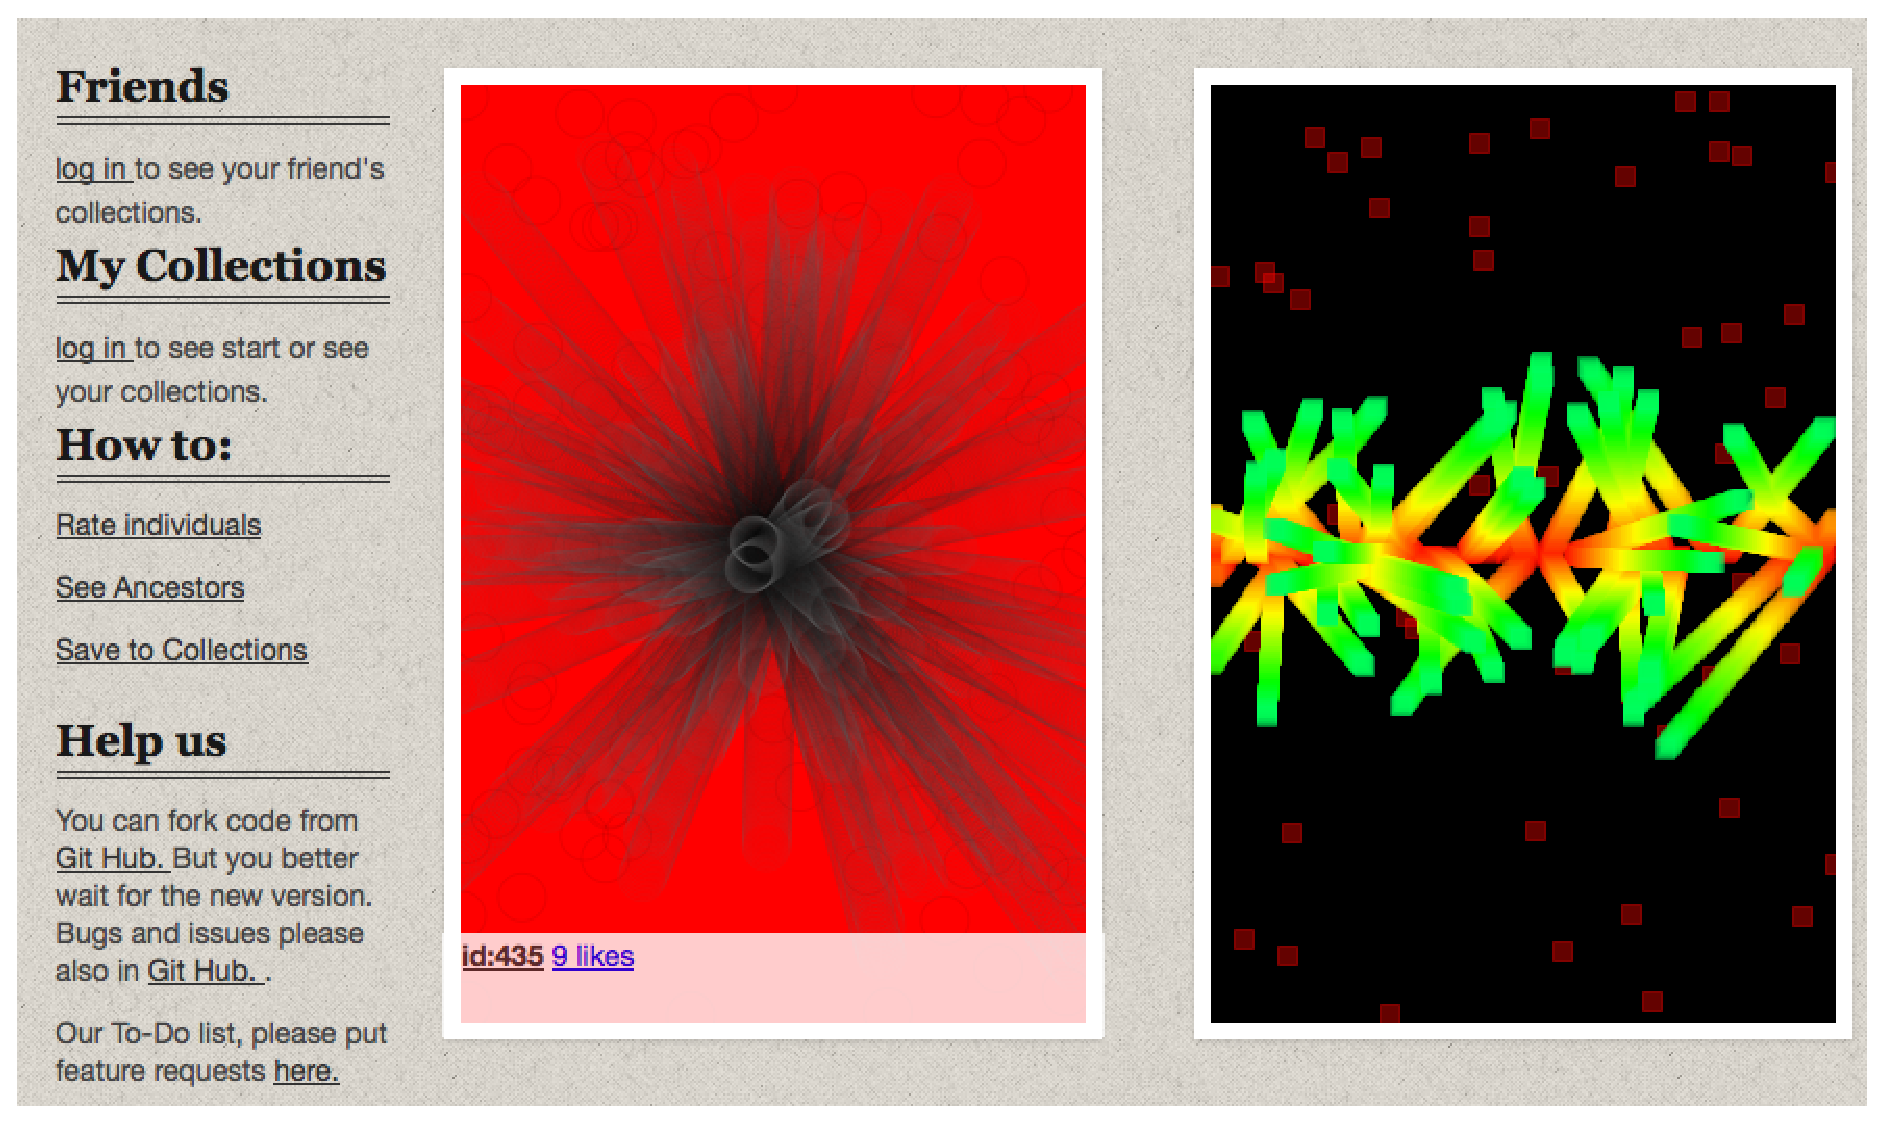
\epsfig{file=shapes.eps, width=3.5in}
  \caption{evoSpace project, Shapes}
  \label{PicShapes}
\end{figure}

\subsection{Article Spinning}

Article spinning is a method used to create multiple versions of a
text article without creating versions considered as plagiarism, due
to the uniqueness achieved of the generated content. Duplicated
content is not accepted by several search engines like Google, Yahoo
and Bing, so this method is used to generate many different versions
of a single article that have a higher probability of being considered
as unique content by these search engines. Words and phrases are
randomly changed by other text blocks that have the same meaning,
resulting in another version of the article with the same meaning, but
different text content \cite{malcolm2008approach}.

\subsection{Related Work}
\label{RelatedWork}

\subsubsection{evoSpace-Interactive}

evoSpace-interactive was initially tested by implementing an
interactive evolutionary computation program called "Shapes''
\cite{garcia2013evospace}. This software evolved images formed by equilateral
triangles that could have one of twelve possible colors. Currently,
EvoSpace has made modifications to the images displayed by changing
the shape to more attractive animations that last for a short period
of time. For this work, we modified evoSpace to be capable of
displaying text ads instead of images.

\section{Methodology}

\subsection{Article Spinning Format}
\label{ArticleSpinning}

The text in Figure \ref{PicArticleSpinning} contains different sections enclosed by curly
braces, which contain different text blocks. These text blocks can be of
arbitrary length, from a single word to whole sentences and
paragraphs. The bars present in the text work as separators,
indicating the algorithm that the text before a bar will represent one
of the possible choices of a combination of text. The text blocks that are outside of
the curly braces (represented by grey text in Figure \ref{PicArticleSpinning}) won't have any
modifications when the texts evolve; they are constant throughout all
the generations of the evolutionary algorithm. The text's structure is very
similar to that used in Article Spinning algorithms.

\begin{figure}
  \centering
  
\epsfig{file=ArticleSpinningFormat.eps, width=3.5in}
  \caption{A sample of an advertisement text in article spinning format}
  \label{PicArticleSpinning}
\end{figure}

The text presented in Figure \ref{PicArticleSpinning} is written in
Spanish, as it's the first language of the participants of the
experiment.

\subsection{Constructed Texts}

At the moment, two advertisement texts have been evolved and tested
against five different versions generated by five different experts
(see Section \ref{TextEfficiency}). The first advertisement is about a
hamburger, and the second advertisement is about an automobile. The results
can be seen in Section \ref{Results}.

\subsection{Evolution of the Texts}
\label{EvolutionProcess}

The texts were evolved for 30 generations, one generation being an
evaluation by an user between two different versions of an
advertisement.

The evolution process consists on the random selection of twelve
chromosomes (i.e., a version of the text), where six chromosomes will
act as possible fathers, and the other six as possible mothers. A
fitness value is calculated for each chromosome, with the following
formula:

\begin{equation}
  f = \frac{s + 1}{v + 1}
\end{equation}

where \textit{f} is the fitness of the chromosome, \textit{s} is the
number of times the chromosome has been selected, and \textit{v} is
the number of times the chromosome has been viewed. The chromosomes
with a low number of views (i.e., 2 views) are exempt from the
evolution process, as it would be too soon to consider them with a low
fitness already. Then, the father and the mother with the highest
fitnesses are chosen, and, according to a probability of crossover
(i.e., 0.8), they will interchange genetic material to produce two
children. Two chromosomes with the lowest fitness will be discarded,
and will be replaced by the offspring of the more fit father and
mother.

Additionally, there's a chance of 2\% for a mutation to occur to the
offspring. This mutation consists on the random alteration of the
genetic material of the chromosomes.

\subsection{evoSpace Adaptation}
\label{EvoSpaceAdaptation}

evoSpace had to be modified in several areas of its programming. A new
module accepts a chromosome as input, and produces a version of the
advertisement text based on it. The front end of the application
changed to be able to display text instead of animations, as in the
Shapes application. The social features of the platform are not shown
in this adaptation, so they don't have the possibility of confusing
the participants in the experiments. Also, the new design allows a
picture to be added in the middle of the template. The purpose of this
picture is to give a general idea of the product being advertised to
the user.

In Figure \ref{PicText}, the adapatation of evoSpace for the evolution
of advertisement texts is shown. Two different versions of the text
are shown to the user in the bottom, a picture of the product being
advertised is shown in the middle, and a button for getting more text
versions is shown in the top right corner.

\begin{figure}
  \centering
  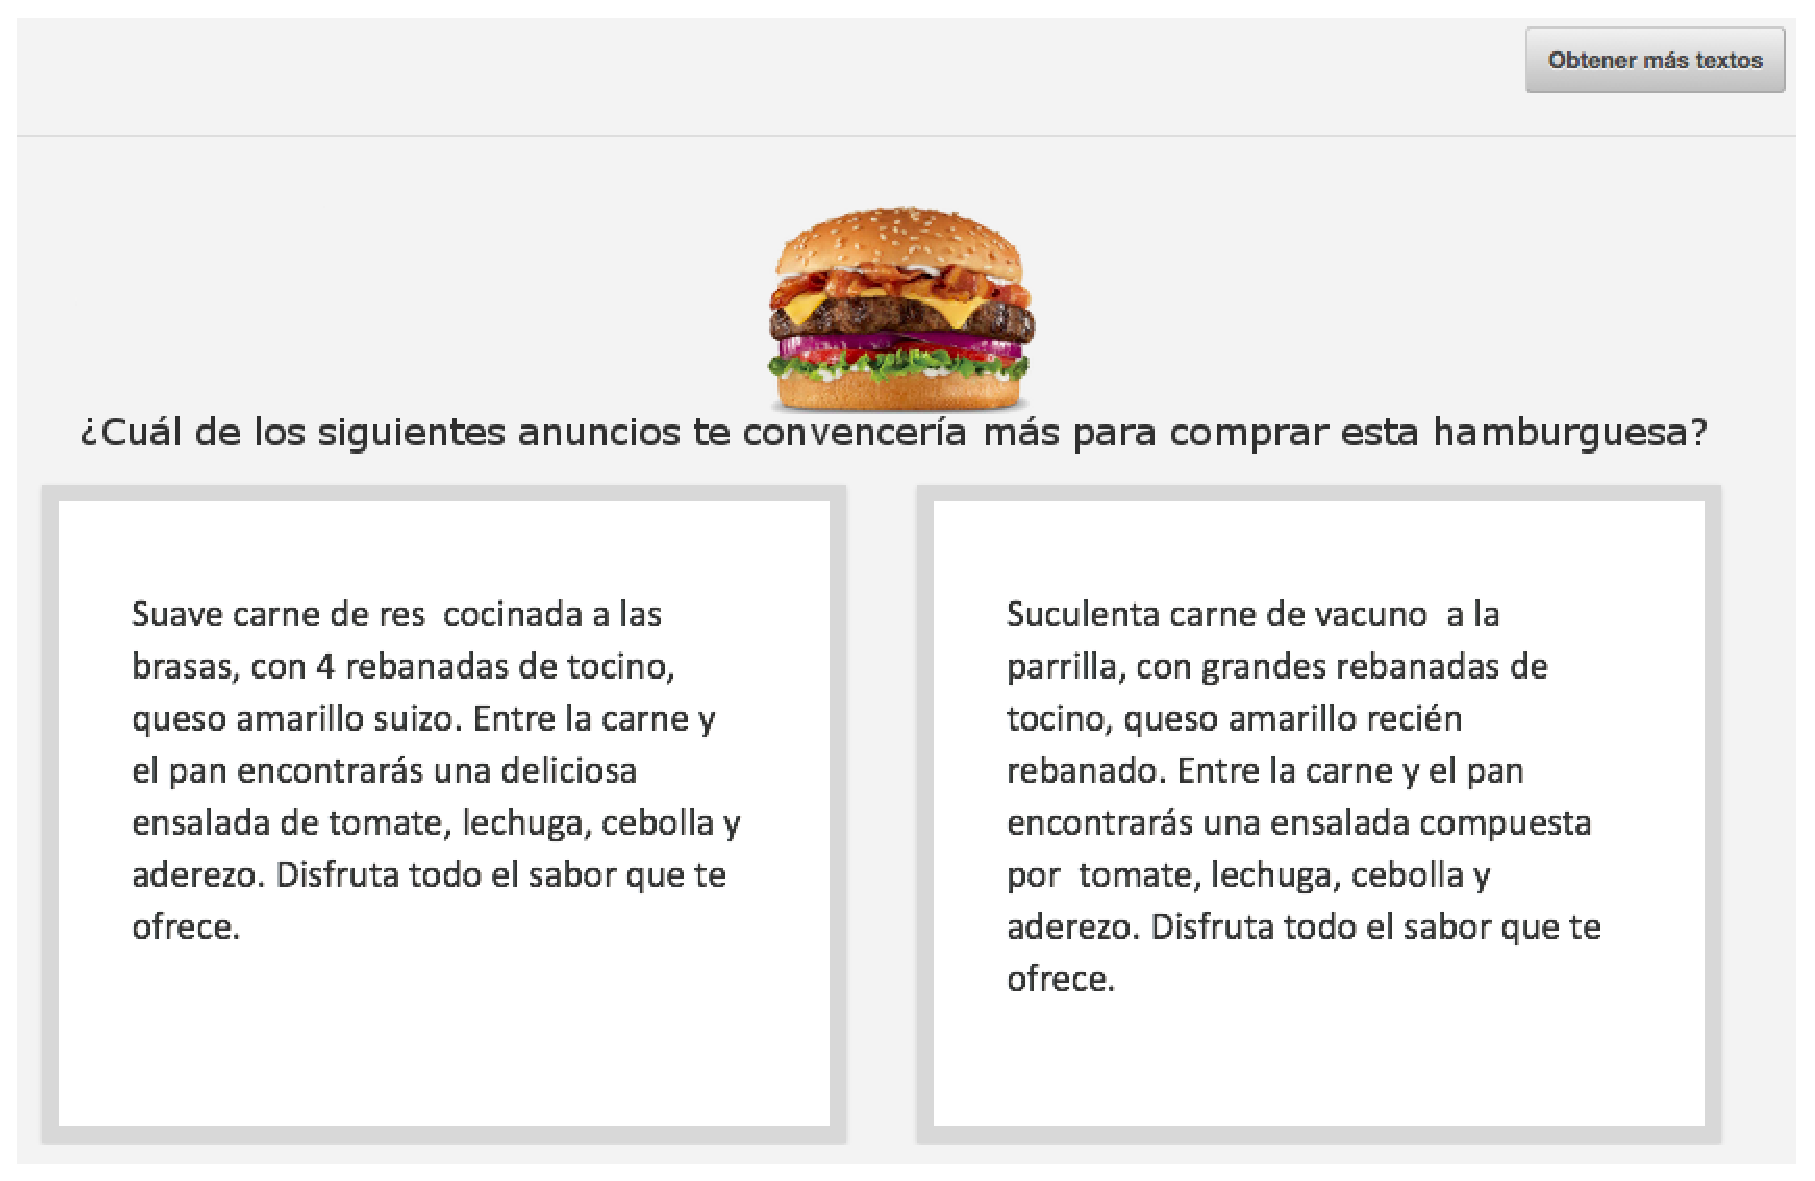
\epsfig{file=text.eps, width=3.5in}
  \caption{Adaptation of evoSpace for the evolution of advertisement texts}
  \label{PicText}
\end{figure}

\subsection{Advertisement Text Efficiency}
\label{TextEfficiency}

Measuring the efficiency of an advertisement text is performed by
comparing a version resulting from the evolution of the texts, against
a version constructed by an expert. For the experiments, any person
specialized in an area related to marketing is considered an expert.

For the first part of the experiment, a group of 30 people, randomly
chosen, are asked to choose what version they think would persuade
them the most. The text with the majority of the votes is then
considered to be the better at persuading a person to buy the
advertised product. Although this test could present flaws, as
the best strategy to measure the effectiveness of an advertisement
text would be to put it in actual practice, the test can produce a
rough idea of the real results.

This part of the experiment is repeated with five different versions
from different experts, against the same evolved text.

For the second part, recall and recognition tests
\ref{RecallRecognition} are performed. The recognition test consists
on showing a group of 30 people a dummy website, where a movie trailer
is played for 30 seconds. Above this video, the advertisement text is
displayed. After the completion of the video, the website is hidden,
and the participants are asked if they saw an advertisement above the
video. If the participants saw the video, this means they recognized
the advertisement. In the end, the number of people who recognized the
text is divided by 30, the total number of participants, and this
represents the percentage of recognition for the given advertisement.

The recall test is performed after the recognition test. The same
group of people that participated in the recognition test, and that
successfully recognized the advertisement, are asked if they recall
what was the subject of the text. Like in the recognition test, the
number of people who recalled the subject of the text is divided by
30, the total number of participants, and this represents the
percentage of recall for the given advertisement.

In Figure \ref{RecallRecognition}, the dummy website is
illustrated. The video can be seen on the right, and the advertisement
text on its top, surrounded with a blue border.

\begin{figure}
  \centering
  
\epsfig{file=RecallRecognition.eps, width=3.5in}
  \caption{Dummy website built for the recognition and recall tests}
  \label{RecallRecognition}
\end{figure}

\subsection{Clustering and Recommendation}
\label{ClusteringRecommendation}

Before an individual interacts with the application developed in
evoSpace-Interactive, a profile of the user is gathered. Using the
users' profiles, user clusters can be created. This allows the IEC
process to be isolated for each of the clusters, thus, creating
different, optimized, versions for each cluster of people. In this
way, a recommendation of an advertisement text can be achieved.

\section{Partial Results}
\label{Results}

Table \ref{Hamburger} presents the results of the experiments conducted
using the hamburger advertisement text, while Table \ref{Automobile}
presents the results of the automobile advertisement text. An
explanation of the experiments can be found in Section
\ref{TextEfficiency}.

The percentages shown in the tables represent the ratings given by the
participants to each advertisement text version. For example, 60/150,
or 60\%, means that 60 people out of the 150 people that participated
in the experiment, successfully recognized or recalled the given
text. In the persuasion test, the results are complementary, meaning
that, for example, 56\% of the participants preferred the evolved
version of the hamburger text, while 44\% of the participants preferred
the expert's choice.

As was mentioned in Section \ref{TextEfficiency}, 30 people
participated for each part of the experiment. 150 different people were needed
for each test, because every part was performed five times (the
evolved text competed against five different experts' choices).

\begin{table}
  \begin{tabular}{| c || c | c |}
    \hline
    Type of Test & Evolved Text Rating & Expert's Text Rating \\ \hline
    Recognition & 60/150 = 40\% & 69/150 = 46\% \\ \hline
    Recall & 41/150 = 27.3\% & 33/150 = 22 \\ \hline
    Persuasion & 84/150 = 56\% & 66/150 = 44\% \\
    \hline
  \end{tabular}
  \caption{Results of the hamburger advertisement experiment}
  \label{Hamburger}
\end{table}

\begin{table}
  \begin{tabular}{| c || c | c |}
    \hline
    Type of Test & Evolved Text Rating & Expert's Text Rating \\ \hline
    Recognition & 98/150 = 65.3\% & 98/150 = 65.3\% \\ \hline
    Recall & 49/150 = 32.6\% & 36/150 = 24\% \\ \hline
    Persuasion & 81/150 = 54\% & 69/150 = 46\% \\
    \hline
  \end{tabular}
  \caption{Results of the automobile advertisement experiment}
  \label{Automobile}
\end{table}

\section{Conclusions}

More and better designed experiments need to be performed in order to
obtain more reliable results. Also, an experiment must be designed to
test the efficacy of the recommendations by the clustering method
proposed in Section \ref{ClusteringRecommendation}.

Although conclusive results have not yet been generated, the partial
results presented in Section \ref{Results} demonstrate that the
proposed method in this work can potentially aid in the development of
a marketing campaign.

\bibliographystyle{abbrv}
\bibliography{sigproc}

\balancecolumns
\end{document}
